\documentclass[pdftex,a4paper,12pt,origdate,french]{supaero-lettre}

\usepackage[utf8]{inputenc}
\usepackage[T1]{fontenc}
\usepackage{ae,aecompl,aeguill}
\usepackage{tikz}
\usepackage{amsmath}
\usepackage[pdfversion=1.7, pdftex, colorlinks, urlcolor=blue, pdfstartview=FitH, pdfhighlight={/N}]{hyperref}
\usepackage{verbatim}

\begin{document}

\begin{letter}{Ausias Gamisans\\ Professeur Associé d'Espagnolo
    Facilo\\ISAE/LACS}

\signature{Christophe Garion\\
           Resp. «~Mise à niveau littéraires~»\\
           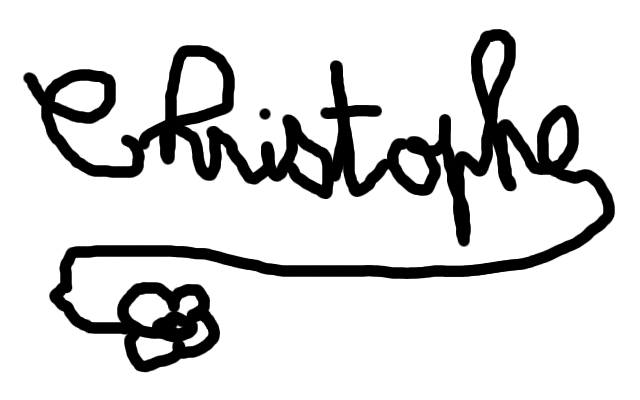
\includegraphics[scale=0.25]{false-sig-tof.png}}

%======================================================================
% Adresse différente, pas de téléphone etc.
%======================================================================
%\address{}
%\telephone{}
%\nofax
%\email{}
%lieu{}
\Nref{2009BLABLA}
%\Vref{}
\conc{notre discussion d'hier}


\opening{Cher Ausias,}

Suite à ta question d'hier, je me permets de t'écrire pour te rappeler
la formulation du théorème de Pythagore. Supposons\footnote{Les
  scientifiques utilisent beaucoup ce mot. C'est pour poser ce que
  l'on appelle une \emph{hypothèse}.} que l'on ait un triangle
rectangle de côtés de longueurs $a$, $b$ et $c$ (les côtés
adjacents\footnote{Adjacent signifie «~à côté de~». Si si,
  souviens-toi, tu as entendu ce mot au collège.} à l'angle droit
étant ceux de longueur $a$ et $b$) comme représenté ci-dessous:

  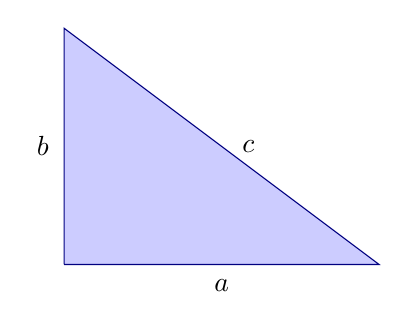
\begin{tikzpicture}
    \filldraw[draw=blue!50!black, fill=blue!20] (0,0) -- 
    node[pos=0.5, color=black, below, yshift=-2pt] {$a$} (4,0) -- 
    node[pos=0.5, color=black, right, xshift=4pt, anchor=west] {$c$}
    (0,3) -- 
    node[color=black, pos=0.5, left, xshift=-2pt] {$b$} (0,0);
  \end{tikzpicture}

  Dans ce cas, l'équation suivante, appelée théorème de Pythagore,
  permet de relier les trois grandeurs $a$, $b$ et $c$:

    \begin{equation}
      \label{eq:1}
      a^2 + b^2 = c^2
    \end{equation}

Dans notre cas, si $a = 4$ et $b = 3$ et que l'on cherche la valeur de
$c$, on peut donc écrire\footnote{Tu peux mesurer la figure précédente
  avec ta règle graduée et trouver la solution, mais ce n'est pas
  l'objectif de l'exercice.}:

\begin{equation*}
  \begin{split}
    c^2 & = 4^2 + 3^2\\
     & = 16 + 9\\
     & = 25\\
    c & = \sqrt{25} \text{ car $c$ est une valeur
      positive\footnotemark}\\
      & = 5
  \end{split}
\end{equation*}

\footnotetext{Souviens-toi, il s'agit d'une longueur!}

Bonus vocabulaire: le côté de longueur $c$ s'appelle
\emph{l'hypoténuse}. Ce n'est pas vrai pour tous les côtés de longueur
$c$, il s'agit en fait du côté qui ne «~touche~» pas l'angle
droit. Dans notre exemple il est de longueur $c$, mais c'est un cas
particulier.

La semaine prochaine, nous parlerons des fractions. C'est un peu
difficile, mais je sens que tu as le potentiel pour bien comprendre
tout cela.

\closing{Amitiés scientifiques,}

% pièces jointes
%\encl{}
\cc{DFS}
\ps{PS:}{je tiens à préciser qu'Ausias Gamisans possède un BAC scientifique
acquis de haute volée et est donc parfaitement au courant de ces
notions.}

\vspace{2cm}

Tu peux maintenant légitimement te demander comment j'ai pu taper
cette magnifique lettre sans Word. J'ai en effet utilisé \LaTeX, un
logiciel de mise en page pour les nains formaticiens et les
scientifiques en général.

La marche à suivre est très simple~: il faut disposer de la classe
\texttt{lettre} (disponible dans la plupart des distributions \LaTeX),
de la classe \texttt{supaero-lettre} que j'ai créée et qui en dérive
et du fichier \texttt{supaero.ins} que tu pourras modifier pour mettre
ton nom, ton propre numéro de téléphone etc. Je te conseille de lire
la documentation du paquetage \texttt{lettre}
(\url{http://www.ctan.org/tex-archive/help/Catalogue/entries/lettre.html}). Toutes
les commandes définies dans \texttt{supaero.ins} peuvent être
redéfinies dans le corps de la lettre pour la personnaliser. Par
exemple, tu trouveras dans la suite une lettre en anglais.

Attention, j'utilise l'option \texttt{origdate} qui permet de
conserver pour la date de la lettre la date de création du fichier. Si
tu veux la modifier, détruis le fichier qui porte le même nom que ton
fichier source mais avec l'extension \texttt{odt}.

Le code source de cette lettre est disponible ci-après. Tu verras donc
que pour les fax, c'est le même principe.

\verbatiminput{exempleLettre.tex}

\end{letter}

\begin{letter}{Ausias Gamisans\\ Associate Professor of Espagnolo Facilo\\ISAE/LACS}

\anglais

\signature{Christophe Garion}

\Nref{2009BLABLA}

\conc{our previous meeting}

\opening{Dear Ausias,}

Blablablablablablablablablabla.

\closing{Sincerely yours,}

\end{letter}

\begin{telefax}{+01-555-7456542}{Bill Gates\\Micro\$oft\\Redmond\\USA}

\conc{qualité des logiciels de votre entreprise}

\opening{Cher M. Gates,}

Je trouve que la qualité de vos logiciels laisse plus qu'à désirer.

\closing{Je ne vous salue pas.}

\end{telefax}
\end{document}
